\chapter{电磁感应}
\section{电磁感应现象 楞次定律}

1.磁通量

(1)定义

匀强磁场中,磁感应强度(B)与\_\_垂直\_\_于磁场方向的面积(S)的乘积叫做穿过这个面积的磁通量,简称磁通,我们可以用穿过这一面积的磁感线条数的多少来形象地理解.

(2)公式

$\Phi=BS.$在国际单位制中,磁通量的单位是\_\_韦伯\_\_,符号是Wb.

(3)磁通密度

垂直穿过单位面积的\_\_磁感线\_\_的条数,叫做磁通密度,即$B=\dfrac{\Phi}{S}$,磁感应强度又称磁通密度.

2.电磁感应现象

(1)产生感应电流的条件

穿过闭合电路的\_\_磁通量\_\_发生变化.

(2)产生感应电动势的条件

无论回路是否闭合,只要穿过线圈平面的\_\_磁通量\_\_发生变化,线圈中就有感应电动势产生,产生感应电动势的那部分导体相当于\_\_电源\_\_.

(3)电磁感应现象的实质

电磁感应现象的实质是产生\_\_感应电动势\_\_,如果电路闭合,则有\_\_感应电流\_\_;如果电路不闭合,则只有\_\_感应电动势\_\_而无感应电流.

3.感应电流方向的判定

(1)右手定则

\ding{172}内容:伸开\_\_右手\_\_,使拇指与其余四指垂直,并且都与手掌在同一平面内,让磁感线从\_\_手心垂直\_\_进入,并使拇指指向\_\_导体运动\_\_的方向,这时四指所指的方向就是\_\_感应电流\_\_的方向.

\ding{173}适用范围:适用于判断闭合电路中的部分导体切割磁感线产生感应电流的情况.

(2)楞次定律

\ding{172}内容,感应电流具有这样的方向,即感应电流的磁场总要\_\_阻碍\_\_引起感应电流的磁通量的变化.

\ding{173}适用情况:所有\_\_电磁感应\_\_现象.
\newpage
\subsection{对电磁感应现象的理解}

1.磁通量发生变化的三种常见情况

(1)磁场强弱不变,回路面积改变.

(2)回路面积不变,磁场强弱改变.

(3)回路面积和磁场强弱均不变,但二者的相对位置发生改变.

2.判断电磁感应现象是否发生的流程

\begin{center}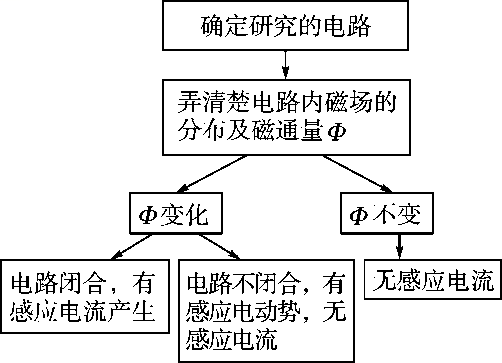
\includegraphics[width=2.28333in,height=1.65069in]{media/image387.png}\end{center}

\newpage
\subsection{感应电流方向的判断}

1.感应电流方向判断的两种方法

方法一 用楞次定律判断

\begin{center}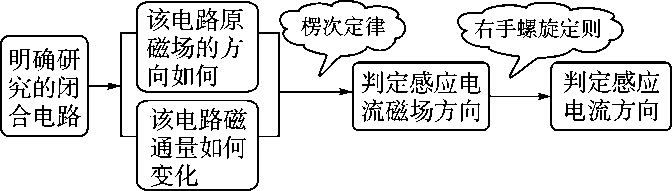
\includegraphics[width=3.05694in,height=0.86806in]{media/image389.png}\end{center}

方法二 用右手定则判断

该方法适用于部分导体切割磁感线.判断时注意掌心、四指、拇指的方向:

(1)掌心------磁感线穿入;

(2)拇指------指向导体运动的方向;

(3)四指------指向感应电流的方向.

2.楞次定律和右手定则的关系

(1)从研究对象上说,楞次定律研究的是整个闭合回路,右手定则研究的是闭合电路中的一部分导体,即一段导体做切割磁感线运动的情况.

(2)从适用范围上说,楞次定律适用于磁通量变化引起感应电流的各种情况(包括一部分导体做切割磁感线运动的情况),右手定则只适用于一段导体在磁场中做切割磁感线运动的情况.因此,右手定则是楞次定律的一种特殊情况.一般来说,若导体不动,回路中磁通量变化,应该用楞次定律判断感应电流方向而不能用右手定则;若是回路中一部分导体做切割磁感线运动产生感应电流,用右手定则判断较为简单,用楞次定律进行判断也可以,但较为麻烦.

\begin{center}
\includegraphics[width=0.70764in,height=0.12292in]{media/image37.png}\end{center}
\begin{center}
	\textbf{应用楞次定律判断感应电流方向的步骤}
\end{center}

\begin{center}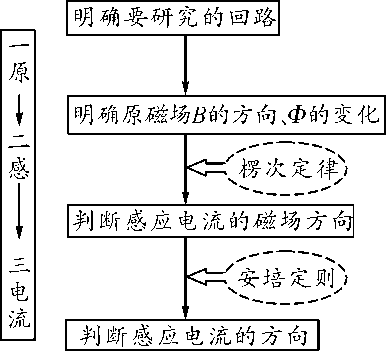
\includegraphics[width=1.75486in,height=1.59444in]{media/image390.png}\end{center}

\newpage
\subsection{楞次定律的推论应用}

楞次定律中``阻碍''的含义可以推广为:感应电流的效果总是阻碍引起感应电流的原因,列表说明如下.

\begin{longtable}[]{@{}m{3cm}m{7cm}@{}}
\toprule
内容 & 例证\tabularnewline
\midrule
\endhead

阻碍原磁通量变化------``增反减同''
& \begin{minipage}[t]{0.47\columnwidth}\raggedright
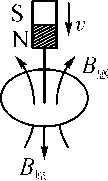
\includegraphics[width=0.49028in,height=0.82083in]{media/image392.png}磁铁靠近线圈,B感与B原反向\strut
\end{minipage}\tabularnewline

阻碍相对运动------``来拒去留''
& \begin{minipage}[t]{0.47\columnwidth}\raggedright
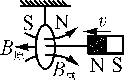
\includegraphics[width=0.56597in,height=0.36806in]{media/image393.png} 磁铁靠近,是斥力

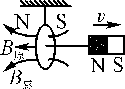
\includegraphics[width=0.56597in,height=0.40556in]{media/image394.png} 磁铁远离,是引力\strut
\end{minipage}\tabularnewline
\multirow{2}{3cm}{使回路面积有扩大或缩小的趋势------``增缩减扩''}
& \begin{minipage}[t]{0.47\columnwidth}\raggedright

	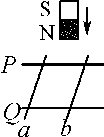
\includegraphics[width=0.47153in,height=0.62292in]{media/image395.png}

P、Q是光滑固定导轨,a、b是可动金属棒,磁铁下移,面积应减小,a、b靠近\strut
\end{minipage}\tabularnewline
&
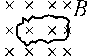
\includegraphics[width=0.39653in,height=0.25486in]{media/image396.png} B减小,线圈扩张\tabularnewline
\bottomrule
\end{longtable}


\subsection{三定则一定律的综合应用}

1.``三定则一定律''的比较

\begin{longtable}[]{@{}m{3cm}m{5cm}m{3cm}@{}}
\toprule
名称 & 基本现象 & 应用的定则或定律\tabularnewline
\midrule
\endhead
电流的磁效应 & 运动电荷、电流产生磁场 & 安培定则\tabularnewline
洛伦兹力、 安培力 & 磁场对运动电荷、电流有作用力 &
左手定则\tabularnewline
\multirow{2}{3cm}{电磁感应} & 部分导体做切割磁感线运动 & 右手定则\tabularnewline
& 闭合回路磁通量变化 & 楞次定律\tabularnewline
\bottomrule
\end{longtable}

\begin{center}
\includegraphics[width=0.70764in,height=0.12292in]{media/image37.png}\end{center}
\begin{center}
	\textbf{三定则、一定律的应用技巧}
\end{center}

(1)应用楞次定律,必然要用到安培定则.

(2)感应电流受到安培力,有时可以先用右手定则确定电流的方向,再用左手定则确定安培力的方向,有时也可以直接应用楞次定律的推论确定安培力的方向.


\newpage
\section{法拉第电磁感应定律 自感现象}

1.法拉第电磁感应定律

(1)感应电动势

\ding{172}概念:在\_\_电磁感应现象\_\_中产生的电动势;

\ding{173}产生条件:穿过回路的\_\_磁通量\_\_发生改变,与电路是否闭合\_\_无关\_\_;

\ding{174}方向判断:感应电动势的方向用\_\_楞次定律\_\_或\_\_右手定则\_\_判断.

(2)法拉第电磁感应定律

\ding{172}内容:感应电动势的大小跟穿过这一电路的\_\_磁通量的变化率\_\_成正比;

\ding{173}公式:$E=n \dfrac{\Delta \Phi}{\Delta t}$,其中n为线圈匝数,$\dfrac{\Delta \Phi}{\Delta t}$为磁通量的\_\_变化率\_\_.

(3)导体切割磁感线时的感应电动势

\ding{172}导体垂直切割磁感线时,感应电动势可用E=Blv求出,式中l为导体切割磁感线的有效长度;

\ding{173}导体棒在磁场中转动时,导体棒以端点为轴,在匀强磁场中垂直于磁感线方向匀速转动产生感应电动势$E=B l \bar{v}=\dfrac{1}{2}Bl^2\omega$.(平均速度等于中点位置的线速度$\dfrac{1}{2} l \omega$)

2.自感、涡流

(1)自感现象

\ding{172}概念:由于导体本身的\_\_电流\_\_变化而产生的电磁感应现象称为自感.

\ding{173}自感电动势

a.定义:在自感现象中产生的\_\_感应电动势\_\_叫做自感电动势;

b.表达式:$E=L \dfrac{\Delta I}{\Delta t}$

\ding{174}自感系数L

a.相关因素:与线圈的\_\_大小\_\_、形状、\_\_匝数\_\_以及是否有铁芯有关;

b.单位:亨利(H),$1 \mathrm{mH}=10^{-3} \mathrm{H}, 1 \mu \mathrm{H}=10^{-6}$.

(2)涡流

当线圈中的电流发生变化时,在它附近的任何导体中都会产生\_\_感应\_\_电流,这种电流像水的漩涡,所以叫涡流.

(3)电磁阻尼

导体在磁场中运动时,感应电流会使导体受到安培力,安培力的方向总是\_\_阻碍\_\_导体的运动.

(4)电磁驱动

如果磁场相对于导体转动,在导体中会产生\_\_感应电流\_\_使导体受到安培力而使导体运动起来.
\newpage
\subsection{对法拉第电磁感应定律的理解}

1.$\Phi$、$\Delta \Phi$、$\dfrac{\Delta \Phi}{\Delta t}$的对比理解

\begin{longtable}[]{@{}m{1.5cm}m{3.7cm}m{3.2cm}m{3.7cm}@{}}
\toprule
比较项 & $\varphi$ & $\Delta \varphi$ &$\dfrac{\Delta \Phi}{\Delta t}$\tabularnewline
\midrule
\endhead
物理意义 & 穿过某一面积的磁通量 & 穿过某一面积的磁通量的变化量 &
穿过某一面积的磁通量的变化率\tabularnewline
大小计算 & $\Phi=BSsin \theta$($\theta$是S与B的夹角) & $\Delta \Phi=\Phi_2-\Phi_1 $&
$\dfrac{\Delta \Phi}{\Delta t}=S \dfrac{\Delta B}{\Delta t}$ 或 $B \dfrac{\Delta S}{\Delta t}$\tabularnewline
注意问题 & 磁感线有穿入和穿出,计算时要抵消 & 穿过的磁通量的方向 &
在$\Phi_­t$图象中用斜率表示\tabularnewline
\bottomrule
\end{longtable}

注意:\ding{172}$\Phi$、$\Delta \Phi$、$\dfrac{\Delta\Phi}{\Delta t}$的大小之间没有必然的联系,$\Phi$,$\dfrac{\Delta\Phi}{\Delta t}$不一定等于0;\ding{173}感应电动势E与线圈匝数n有关,但$\Phi$、$\Delta \Phi$、$\dfrac{\Delta\Phi}{\Delta t}$的大小均与线圈匝数无关.

2.法拉第电磁磁应定律应用的三种情况

(1)磁通量的变化是由面积变化引起时,$\Delta \Phi=B\Delta S$,则$E=n \dfrac{B \Delta S}{\Delta t}$. 

(2)磁通量的变化是由磁场变化引起时,$\Delta \Phi \neq BS$,则$E=n \dfrac{ \Delta BS}{\Delta t}$,S是磁场范围内的有效面积.

(3)磁通量的变化是由于面积和磁场变化共同引起的,则根据定义求,$\Delta \Phi=\Phi_{\text {末 }}-\Phi_{\text {初 }}, E=n \dfrac{B_{2} S_{2}-B_{1} S_{1}}{\Delta t} \neq n \dfrac{\Delta B \Delta S}{\Delta t}$

\begin{center}
\includegraphics[width=0.70764in,height=0.12292in]{media/image34.png}\end{center}
\begin{center}
	\textbf{应用法拉第电磁感应定律$E=n \dfrac{\Delta \Phi}{\Delta t}$时应注意}
\end{center}


(1)研究对象:$E=n \dfrac{\Delta \Phi}{\Delta t}$的研究对象是一个回路,而不是一段导体.

(2)物理意义:由$E=n \dfrac{\Delta \Phi}{\Delta t}$求的是$\Delta$t时间内的平均感应电动势,当$\Delta$t$\rightarrow$0时,则E为瞬时感应电动势.

(3)由$E=n \dfrac{\Delta \Phi}{\Delta t}$求得的电动势是整个回路的感应电动势,而不是回路中某段导体的电动势,整个回路的电动势为零,其回路中某段导体的感应电动势不一定为零.

\newpage
\subsection{导体切割磁感线产生感应电动势}

1.导体平动切割磁感线

对于导体平动切割磁感线产生感应电动势的计算式E=Blv,应从以下几个方面理解和掌握.

(1)正交性:该公式适用于匀强磁场,且B、l、v三者两两垂直,若三者中任意二者平行,则导体都不切割磁感线,E=0.

(2)平均性:导体平动切割磁感线时,若v为平均速度,则$\bar E$为平均感应电动势,即$\bar E =Bl\bar v$.

(3)瞬时性:若v为瞬时速度,则E为相应的瞬时感应电动势.

(4)有效性:公式中的l为有效切割长度,即导体在与v垂直的方向上的投影长度.下表为常见切割情景中的有效长度.

\begin{longtable}[]{@{}m{1cm}m{2.5cm}m{6cm}@{}}
\toprule
情景 & 图示 & 有效长度说明\tabularnewline
\midrule
\endhead
情景1 &
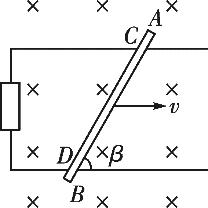
\includegraphics[width=0.94306in,height=0.94306in]{media/image407.png} &
有效长度为l=CDsin $\beta$(容易出现有效长度l=ABsin $\beta$的错误)\tabularnewline
\begin{minipage}[t]{0.30\columnwidth}\raggedright
情景2\strut
\end{minipage} & \begin{minipage}[t]{0.30\columnwidth}\raggedright
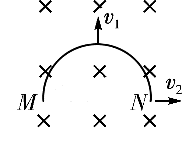
\includegraphics[width=0.85833in,height=0.65069in]{media/image408.png}\strut
\end{minipage} &
\ding{172}沿$v_1$方向运动时,有效长度为l=MN

\ding{173}沿$v_2$方向运动时,有效长度为l=0
\tabularnewline
\begin{minipage}[t]{0.30\columnwidth}\raggedright
情景3\strut
\end{minipage} & \begin{minipage}[t]{0.30\columnwidth}\raggedright
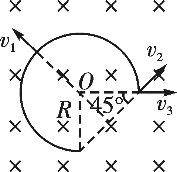
\includegraphics[width=0.80208in,height=0.78333in]{media/image409.png}\strut
\end{minipage} &
\ding{172}沿$v_1$方向运动时,有效长度为l=R

\ding{173}沿$v_2$方向运动时,有效长度为l=0

\ding{174}沿$v_3$方向运动时,有效长度为l=R
\tabularnewline
情景4 &
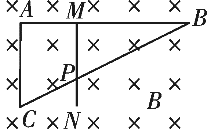
\includegraphics[width=0.94306in,height=0.58472in]{media/image410.png} &
导体棒水平运动切割磁感线的有效长度为导体棒与框架两交点间的距离\tabularnewline
情景5 &
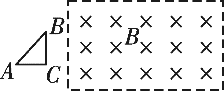
\includegraphics[width=1.01875in,height=0.41528in]{media/image411.png} &
线框ABC水平向右运动进入磁场的过程中,其切割磁感线的有效长度为线框与磁场左边界两交点间的距离\tabularnewline
\bottomrule
\end{longtable}

\begin{center}
\includegraphics[width=0.70764in,height=0.12292in]{media/image13.png}\end{center}
\begin{center}
	\textbf{公式$E=Blv$与公式$E=n \dfrac{\Delta \Phi}{\Delta t}$的比较}
\end{center}

\begin{longtable}[]{@{}m{1cm}m{6cm}m{5cm}@{}}
\toprule
& $E=n \dfrac{\Delta \Phi}{\Delta t}$ & $E=Blv$\tabularnewline
\midrule
\endhead
导体 & 一个回路 & 一段导体\tabularnewline
适用 & 普遍使用 & 导体切割磁感线\tabularnewline
意义 & 常常用于求平均电动势&既可求平均值也可求瞬时值\tabularnewline
联系 & \multicolumn{2}{l}{\shortstack{本质上是统一的.后者是前者的一种特殊情况.但是,当导体做切割磁感线运动时,\\用E=Blv求E比较方便;当穿过电路的磁通量发生变化时,用$E=n \dfrac{\Delta \Phi}{\Delta t}$求E比较方便}}\tabularnewline
\bottomrule
\end{longtable}

\newpage
2.导体转动切割磁感线

当导体在垂直于磁场的平面内,绕一端以角速度$\omega$匀速转动时,产生的感应电动势为$E=B \bar{\nu}=\dfrac{1}{2} B l^{2} \omega$,如图所示.

\begin{center}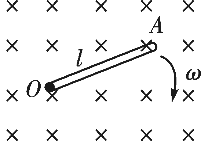
\includegraphics[width=0.91528in,height=0.64167in]{media/image413.png}\end{center}

(1)以中点为轴时,E=0(相同两段的代数和);

(2)以端点为轴时,$E=\dfrac{1}{2} B l^{2} \omega$(平均速度取中点位置时的线速度$\dfrac{1}{2}\omega l$);

(3)以任意点为轴时,$E=\dfrac{1}{2} B \omega\left(l_{1}^{2}-l_{2}\right)$(不同两段的代数和).

\begin{center}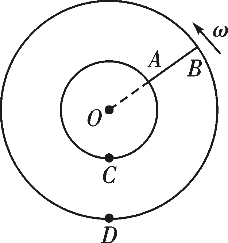
\includegraphics[width=1.0375in,height=1.10347in]{media/image414.png}\end{center}


\subsection{自感现象}

1.自感现象``阻碍''作用的理解

(1)流过线圈的电流增加时,线圈中产生的自感电动势与电流方向相反,阻碍电流的增加,使其缓慢地增加.

(2)流过线圈的电流减小时,线圈中产生的自感电动势与电流方向相同,阻碍电流的减小,使其缓慢地减小.

2.自感现象的四个特点

(1)自感电动势总是阻碍导体中原电流的变化.

(2)通过线圈中的电流不能发生突变,只能缓慢变化.

(3)电流稳定时,自感线圈就相当于普通导体.

(4)线圈的自感系数越大,自感现象越明显,自感电动势只是延缓了过程的进行,但它不能使过程停止,更不能使过程反向.

3.自感现象中的能量转化

通电自感中,电能转化为磁场能;断电自感中,磁场能转化为电能.

\begin{center}
\includegraphics[width=0.70764in,height=0.12292in]{media/image37.png}\end{center}
\begin{center}
	\textbf{分析自感现象的两点注意}
\end{center}

(1)通过自感线圈中的电流不能发生突变,即通电过程中,电流是逐渐变大,断电过程中,电流是逐渐变小,此时线圈可等效为``电源'',该``电源''与其他电路元件形成回路.

(2)断电自感现象中灯泡是否``闪亮''问题的判断,在于对电流大小的分析,若断电后通过灯泡的电流比原来强,则灯泡先闪亮后再慢慢熄灭.


\newpage
\section{电磁感应定律的综合应用}

1.电磁感应中的电路问题

在电磁感应中,切割磁感线的导体或磁通量发生变化的回路将产生\_\_感应电动势\_\_,该导体或回路相当于\_\_电源\_\_.因此,电磁感应问题往往又和电路问题联系在一起.

解决与电路相联系的电磁感应问题的基本方法如下:

(1)用法拉第电磁感应定律和楞次定律(右手定则)确定感应电动势的\_\_大小\_\_和\_\_方向\_\_.

(2)画等效电路图.

(3)运用闭合电路欧姆定律、串并联电路的规律、电功率等公式联立求解.

2.电磁感应中的动力学问题

(1)导体棒的两种运动状态

\ding{172}平衡状态------导体棒处于静止状态或匀速直线运动状态,加速度为\_\_零\_\_;

\ding{173}非平衡状态------导体棒的加速度不为零.

(2)两个研究对象及其关系

电磁感应中导体棒既可看作电学对象(因为它相当于电源),又可看作力学对象(因为有感应电流而受到安培力),而感应电流I和导体棒的\_\_速度v\_\_是联系这两个对象的纽带.

(3)电磁感应中的动力学问题分析思路

\ding{172}电路分析:切割磁感线的导体棒相当于\_\_电源\_\_,感应电动势相当于电源的电动势,导体棒的电阻相当于电源的内阻,感应电流$I=\dfrac{B l v}{R+r}$.  

\ding{173}受力分析:导体棒受到安培力及其他力,安培力$F_{\text {安 }}=B I l=\dfrac{B^{2} l^{2} v}{R+r}$,根据牛顿第二定律列动力学方程$F_{\text{合}}=ma$.

\ding{174}过程分析:由于安培力是变力,导体棒做变加速运动或\_\_变减速\_\_运动,当加速度为零时,达到稳定状态,最后做匀速直线运动,根据共点力的平衡条件列方程$F_{\text{合}}=0$.
\newpage
\subsection{电磁感应中的电路问题}

对电磁感应电源的理解

(1)电源的正负极可用右手定则或楞次定律判定,要特别注意应用``在内电路中电流由负极到正极''这一规律进行判定.

(2)电磁感应电路中的电源与恒定电流的电路中的电源不同,前者是由于导体切割磁感线产生的,公式为E=Blv,其大小可能变化,变化情况可根据其运动情况判断;而后者的电源电动势在电路分析中认为是不变的.

(3)在电磁感应电路中,相当于电源的导体(或线圈)两端的电压与恒定电流的电路中电源两端的电压一样,等于路端电压,而不等于电动势,除非切割磁感线的导体或线圈电阻为零.

(4)在外电路电流由正极经电阻流到负极,电流经电阻R产生电势降落U=IR.

\begin{center}
\includegraphics[width=0.70764in,height=0.12292in]{media/image37.png}\end{center}
\begin{center}
	\textbf{解决电磁感应中电路问题的三部曲}
\end{center}

(1)确定电源

切割磁感线的导体或磁通量发生变化的回路将产生感应电动势,该导体或回路就相当于电源,利用$E=n \dfrac{\Delta \Phi}{\Delta t}$或E=Blv求感应电动势的大小,利用右手定则或楞次定律判断电流方向.如果在一个电路中切割磁感线的有几个部分但又相互联系,可视为等效电源的串、并联.

(2)识别电路结构、画出等效电路

分析电路结构,即分清等效电源和外电路及外电路的串并联关系、判断等效电源的正负极或电势的高低等.

(3)利用电路规律求解

一般是综合应用欧姆定律、串并联电路特点、电容器充电及放电特点、电功和电功率的知识、法拉第电磁感应定律等列方程求解.
\newpage
\subsection{电磁感应中的动力学问题}

电磁感应现象中产生的感应电流在磁场中受到安培力的作用,从而影响导体棒(或线圈)的受力情况和运动情况.

1.两种状态及处理方法

\begin{longtable}[]{@{}lll@{}}
\toprule
状态 & 特征 & 处理方法\tabularnewline
\midrule
\endhead
平衡态 & 加速度为零 & 根据平衡条件列式分析\tabularnewline
非平衡态 & 加速度不为零 &
根据牛顿第二定律进行动态分析或结合功能关系进行分析\tabularnewline
\bottomrule
\end{longtable}

2.力学对象和电学对象的相互关系

\begin{center}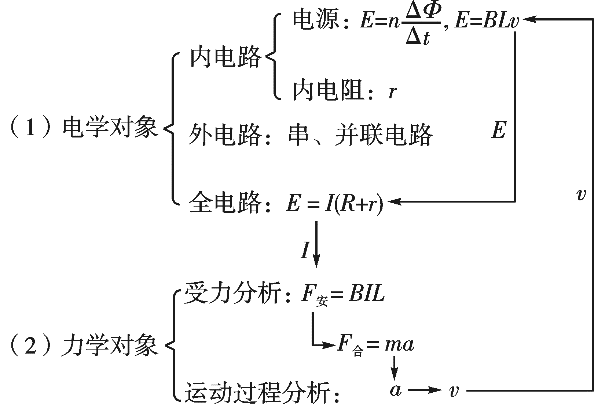
\includegraphics[width=2.69792in,height=1.83958in]{media/image427.png}\end{center}

3.动态分析的基本思路

导体受外力运动$\xlongrightarrow{E=Blv}$感应电动势$\xlongrightarrow{I=\dfrac{E}{R+r}}$感应电流$\xlongrightarrow{F=BIL}$导体受安培力$\rightarrow$合力变化$\xlongrightarrow{F_\text{合}=ma}$加速度变化$\rightarrow$速度变化$\rightarrow$临界状态.

\begin{center}
\includegraphics[width=0.70764in,height=0.12292in]{media/image37.png}\end{center}
\begin{center}
	\textbf{``四步法''分析电磁感应中的动力学问题}
\end{center}

解决电磁感应中动力学问题的一般思路是``先电后力'',具体思路如下:

\begin{center}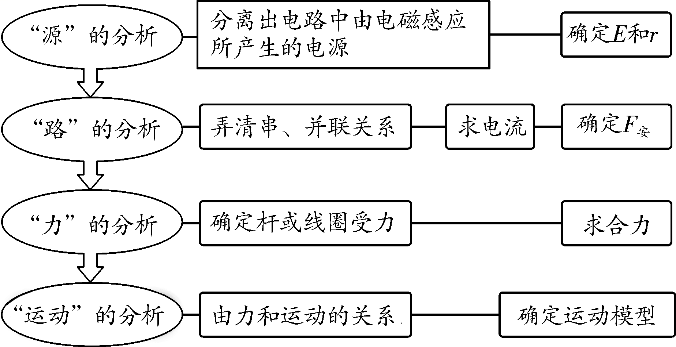
\includegraphics[width=3.07569in,height=1.57569in]{media/image428.png}\end{center}


\newpage
\subsection{电磁感应中的能量问题}

1.电磁感应中的能量转化
(1)安培力做正功:电能$\xlongrightarrow{\text{转化}}$机械能,如电动机
(2)安培力做负功:机械能$\xlongrightarrow{\text{转化}}$电能$\xlongrightarrow[\text{做功}]{\text{电流}}$焦耳热或其他形式的能量,如发电机

2.求解焦耳热Q的三种方法

\begin{center}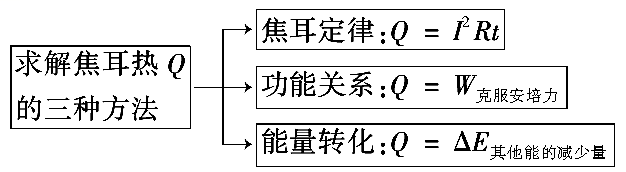
\includegraphics[width=2.71667in,height=0.74514in]{media/image430.png}\end{center}

{[}例3{]}(2018·浙江宁波模拟)如图所示,有一个上、下两层连通且均与水平面平行的``U''型的光滑金属平行导轨,在导轨面上各放一根完全相同的质量为m的匀质金属杆$A_1$和$A_2$,开始时两根金属杆与轨道垂直,在``U''型导轨的右侧空间存在磁感应强度大小为B、方向竖直向上的匀强磁场,杆$A_1$在磁场中,杆$A_2$在磁场之外.设两导轨面相距为H,平行导轨宽为L,导轨足够长且电阻不计,金属杆单位长度的电阻为r.现在有同样的金属杆$A_3$从左侧半圆形轨道的中点从静止开始下滑,在下面与金属杆$A_2$发生碰撞,设碰撞后两杆立刻黏在一起并向右运动.求:

\begin{center}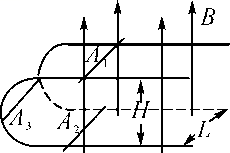
\includegraphics[width=1.04722in,height=0.69792in]{media/image431.png}\end{center}

(1)回路内感应电流的最大值;

(2)在整个运动过程中,感应电流最多产生的热量;

(3)当杆$A_2$、$A_3$与杆$A_1$的速度之比为3:1时,$A_1$受到的安培力大小.
\begin{solution}
	(1)$\dfrac{B \sqrt{g H}}{3 r}$(2)$\dfrac{1}{12} m g H$ (3)$\dfrac{4 B^{2} L \sqrt{g H}}{21 r}$
\end{solution}

\begin{center}
\includegraphics[width=0.70764in,height=0.12292in]{media/image13.png}\end{center}
\begin{center}
	\textbf{解决电磁感应现象中能量问题的一般步骤}
\end{center}

(1)在电磁感应中,切割磁感线的导体或磁通量发生变化的回路将产生感应电动势,该导体或回路就相当于电源.

(2)分析清楚有哪些力做功,就可以知道有哪些形式的能量发生了相互转化.

(3)根据能量守恒列方程求解.

